\documentclass[preview]{standalone}
\usepackage{tikz}
\usetikzlibrary{decorations.pathmorphing, shapes.geometric}

\RequirePackage{amsmath,amsfonts,amssymb}
% Definición de colores personalizados
\definecolor{primaryColor}{RGB}{20,45,105} % color primario
\definecolor{secondaryColor}{RGB}{0,100,160} % Color secundario

\begin{document}
% ============================================================================
% SLIDE 9: Reconstrucción Algorítmica de Jets
% ============================================================================
            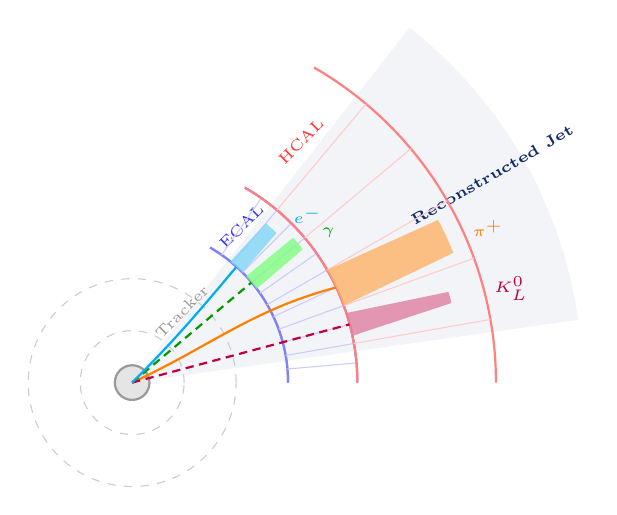
\begin{tikzpicture}[scale=1.1, transform shape]
                
                % 1. CONO DEL JET (Fondo agrupador)
                \fill[primaryColor!10, opacity=0.5] (0,0) -- (52:5.2) arc (52:8:5.2) -- cycle;
                \node[primaryColor, rotate=30] at (30:4.8) {\tiny \textbf{Reconstructed Jet}};
                
                % 2. ESTRUCTURA DEL DETECTOR CMS (Rebanada Transversal)
                % Beam pipe
                \draw[thick, gray!80, fill=gray!20] (0,0) circle (0.2cm);
                
                % Tracker (Capas de silicio concéntricas)
                \draw[gray!40, dashed] (0,0) circle (0.6cm);
                \draw[gray!40, dashed] (0,0) circle (1.2cm);
                \draw[thick, gray!60] (0:1.8) arc (0:60:1.8);
                \node[gray!80, rotate=45] at (55:1.0) {\tiny Tracker};

                % ECAL (Calorímetro Electromagnético)
                \draw[thick, blue!50] (0:1.8) arc (0:60:1.8);
                \draw[thick, blue!50] (0:2.6) arc (0:60:2.6);
                \node[blue!80, rotate=45] at (55:2.2) {\tiny ECAL};
                % Divisiones del ECAL
                \foreach \a in {5,10,...,55} { \draw[blue!20] (\a:1.8) -- (\a:2.6); }

                % HCAL (Calorímetro Hadrónico)
                \draw[thick, red!50] (0:2.6) arc (0:60:2.6);
                \draw[thick, red!50] (0:4.2) arc (0:60:4.2);
                \node[red!80, rotate=45] at (55:3.4) {\tiny HCAL};
                % Divisiones del HCAL (Más gruesas)
                \foreach \a in {10,20,...,50} { \draw[red!20] (\a:2.6) -- (\a:4.2); }

                % 3. FIRMAS DE PARTÍCULAS (Particle Flow Algorithm)
                
                % A) Hadrón Cargado (ej. pion+) -> Traza curva + Shower en HCAL
                \draw[thick, orange] (0,0) to[out=25, in=195] (25:2.6);
                \fill[orange!60, opacity=0.8] (20:2.6) arc (20:30:2.6) -- (28:4.0) arc (28:22:4.0) -- cycle;
                \node[right, orange] at (25:4.2) {\tiny $\pi^+$};
                
                % B) Fotón -> Línea recta punteada + Shower en ECAL
                \draw[thick, green!60!black, densely dashed] (0,0) -- (40:1.8);
                \fill[green!50, opacity=0.8] (37:1.8) arc (37:43:1.8) -- (42:2.5) arc (42:38:2.5) -- cycle;
                \node[right, green!60!black] at (40:2.7) {\tiny $\gamma$};
                
                % C) Hadrón Neutro (ej. Kaon L) -> Línea recta punteada + Shower en HCAL
                \draw[thick, purple, densely dashed] (0,0) -- (15:2.6);
                \fill[purple!50, opacity=0.8] (12:2.6) arc (12:18:2.6) -- (16:3.8) arc (16:14:3.8) -- cycle;
                \node[right, purple] at (15:4.2) {\tiny $K^0_L$};
                
                % D) Electrón -> Traza muy curva + Shower en ECAL
                \draw[thick, cyan] (0,0) to[out=45, in=230] (48:1.8);
                \fill[cyan!50, opacity=0.8] (45:1.8) arc (45:51:1.8) -- (50:2.4) arc (50:46:2.4) -- cycle;
                \node[right, cyan] at (48:2.6) {\tiny $e^-$};
                
            \end{tikzpicture}
\end{document}